% Options for packages loaded elsewhere
\PassOptionsToPackage{unicode}{hyperref}
\PassOptionsToPackage{hyphens}{url}
%
\documentclass[
]{book}
\usepackage{amsmath,amssymb}
\usepackage{iftex}
\ifPDFTeX
  \usepackage[T1]{fontenc}
  \usepackage[utf8]{inputenc}
  \usepackage{textcomp} % provide euro and other symbols
\else % if luatex or xetex
  \usepackage{unicode-math} % this also loads fontspec
  \defaultfontfeatures{Scale=MatchLowercase}
  \defaultfontfeatures[\rmfamily]{Ligatures=TeX,Scale=1}
\fi
\usepackage{lmodern}
\ifPDFTeX\else
  % xetex/luatex font selection
\fi
% Use upquote if available, for straight quotes in verbatim environments
\IfFileExists{upquote.sty}{\usepackage{upquote}}{}
\IfFileExists{microtype.sty}{% use microtype if available
  \usepackage[]{microtype}
  \UseMicrotypeSet[protrusion]{basicmath} % disable protrusion for tt fonts
}{}
\makeatletter
\@ifundefined{KOMAClassName}{% if non-KOMA class
  \IfFileExists{parskip.sty}{%
    \usepackage{parskip}
  }{% else
    \setlength{\parindent}{0pt}
    \setlength{\parskip}{6pt plus 2pt minus 1pt}}
}{% if KOMA class
  \KOMAoptions{parskip=half}}
\makeatother
\usepackage{xcolor}
\usepackage{color}
\usepackage{fancyvrb}
\newcommand{\VerbBar}{|}
\newcommand{\VERB}{\Verb[commandchars=\\\{\}]}
\DefineVerbatimEnvironment{Highlighting}{Verbatim}{commandchars=\\\{\}}
% Add ',fontsize=\small' for more characters per line
\usepackage{framed}
\definecolor{shadecolor}{RGB}{248,248,248}
\newenvironment{Shaded}{\begin{snugshade}}{\end{snugshade}}
\newcommand{\AlertTok}[1]{\textcolor[rgb]{0.94,0.16,0.16}{#1}}
\newcommand{\AnnotationTok}[1]{\textcolor[rgb]{0.56,0.35,0.01}{\textbf{\textit{#1}}}}
\newcommand{\AttributeTok}[1]{\textcolor[rgb]{0.13,0.29,0.53}{#1}}
\newcommand{\BaseNTok}[1]{\textcolor[rgb]{0.00,0.00,0.81}{#1}}
\newcommand{\BuiltInTok}[1]{#1}
\newcommand{\CharTok}[1]{\textcolor[rgb]{0.31,0.60,0.02}{#1}}
\newcommand{\CommentTok}[1]{\textcolor[rgb]{0.56,0.35,0.01}{\textit{#1}}}
\newcommand{\CommentVarTok}[1]{\textcolor[rgb]{0.56,0.35,0.01}{\textbf{\textit{#1}}}}
\newcommand{\ConstantTok}[1]{\textcolor[rgb]{0.56,0.35,0.01}{#1}}
\newcommand{\ControlFlowTok}[1]{\textcolor[rgb]{0.13,0.29,0.53}{\textbf{#1}}}
\newcommand{\DataTypeTok}[1]{\textcolor[rgb]{0.13,0.29,0.53}{#1}}
\newcommand{\DecValTok}[1]{\textcolor[rgb]{0.00,0.00,0.81}{#1}}
\newcommand{\DocumentationTok}[1]{\textcolor[rgb]{0.56,0.35,0.01}{\textbf{\textit{#1}}}}
\newcommand{\ErrorTok}[1]{\textcolor[rgb]{0.64,0.00,0.00}{\textbf{#1}}}
\newcommand{\ExtensionTok}[1]{#1}
\newcommand{\FloatTok}[1]{\textcolor[rgb]{0.00,0.00,0.81}{#1}}
\newcommand{\FunctionTok}[1]{\textcolor[rgb]{0.13,0.29,0.53}{\textbf{#1}}}
\newcommand{\ImportTok}[1]{#1}
\newcommand{\InformationTok}[1]{\textcolor[rgb]{0.56,0.35,0.01}{\textbf{\textit{#1}}}}
\newcommand{\KeywordTok}[1]{\textcolor[rgb]{0.13,0.29,0.53}{\textbf{#1}}}
\newcommand{\NormalTok}[1]{#1}
\newcommand{\OperatorTok}[1]{\textcolor[rgb]{0.81,0.36,0.00}{\textbf{#1}}}
\newcommand{\OtherTok}[1]{\textcolor[rgb]{0.56,0.35,0.01}{#1}}
\newcommand{\PreprocessorTok}[1]{\textcolor[rgb]{0.56,0.35,0.01}{\textit{#1}}}
\newcommand{\RegionMarkerTok}[1]{#1}
\newcommand{\SpecialCharTok}[1]{\textcolor[rgb]{0.81,0.36,0.00}{\textbf{#1}}}
\newcommand{\SpecialStringTok}[1]{\textcolor[rgb]{0.31,0.60,0.02}{#1}}
\newcommand{\StringTok}[1]{\textcolor[rgb]{0.31,0.60,0.02}{#1}}
\newcommand{\VariableTok}[1]{\textcolor[rgb]{0.00,0.00,0.00}{#1}}
\newcommand{\VerbatimStringTok}[1]{\textcolor[rgb]{0.31,0.60,0.02}{#1}}
\newcommand{\WarningTok}[1]{\textcolor[rgb]{0.56,0.35,0.01}{\textbf{\textit{#1}}}}
\usepackage{longtable,booktabs,array}
\usepackage{calc} % for calculating minipage widths
% Correct order of tables after \paragraph or \subparagraph
\usepackage{etoolbox}
\makeatletter
\patchcmd\longtable{\par}{\if@noskipsec\mbox{}\fi\par}{}{}
\makeatother
% Allow footnotes in longtable head/foot
\IfFileExists{footnotehyper.sty}{\usepackage{footnotehyper}}{\usepackage{footnote}}
\makesavenoteenv{longtable}
\usepackage{graphicx}
\makeatletter
\def\maxwidth{\ifdim\Gin@nat@width>\linewidth\linewidth\else\Gin@nat@width\fi}
\def\maxheight{\ifdim\Gin@nat@height>\textheight\textheight\else\Gin@nat@height\fi}
\makeatother
% Scale images if necessary, so that they will not overflow the page
% margins by default, and it is still possible to overwrite the defaults
% using explicit options in \includegraphics[width, height, ...]{}
\setkeys{Gin}{width=\maxwidth,height=\maxheight,keepaspectratio}
% Set default figure placement to htbp
\makeatletter
\def\fps@figure{htbp}
\makeatother
\setlength{\emergencystretch}{3em} % prevent overfull lines
\providecommand{\tightlist}{%
  \setlength{\itemsep}{0pt}\setlength{\parskip}{0pt}}
\setcounter{secnumdepth}{5}
\usepackage{booktabs}
\ifLuaTeX
  \usepackage{selnolig}  % disable illegal ligatures
\fi
\usepackage[]{natbib}
\bibliographystyle{plainnat}
\usepackage{bookmark}
\IfFileExists{xurl.sty}{\usepackage{xurl}}{} % add URL line breaks if available
\urlstyle{same}
\hypersetup{
  pdftitle={DDKtor-DBS SOP},
  pdfauthor={Peter M. Grund, BS},
  hidelinks,
  pdfcreator={LaTeX via pandoc}}

\title{DDKtor-DBS SOP}
\author{Peter M. Grund, BS}
\date{2025-04-16}

\begin{document}
\maketitle

{
\setcounter{tocdepth}{1}
\tableofcontents
}
\chapter{About this SOP}\label{about-this-sop}

\section{Purpose}\label{purpose}

The purpose of this SOP is to provide a description of how to analyze speech data using DDKtor-DBS. DDKtor-DBS, which is a modified version of the original DDKtor program, is a software package that calculates voice onset time (VOT) and vowel duration from diadochokinetic speech task (DDK) recordings. DDK tasks are used to assess speech motor control and are commonly used in patients with essential tremor, Parkinson's disease, and other movement disorders. This SOP is intended for researchers who are interested in using DDKtor-DBS to analyze speech data. It provides a step-by-step guide to using the software, including how to install the software, prepare the data for analysis, run the analysis, and clean the output data.

The SOP is written specifically for members of the University of Minnesota \href{https://nmrc.umn.edu}{Neuromodulation Research Center} (NMRC), \href{https://neuromod.umn.edu/}{Neuromodulation Research and Technology Laboratory} (NRTL), and \href{https://med.umn.edu/neurology}{Department of Neurology}, but it can be adapted for use by other researchers. The SOP assumes that the reader has a basic understanding of speech analysis and is familiar with the Python programming language. It also assumes that the reader has access to a Linux or Mac computer and is comfortable using the command line. Windows users may need to adapt some of the instructions to work on their system.

Questions about this SOP should be directed to Peter M. Grund, BS, at \href{mailto:grund130@umn.edu}{\nolinkurl{grund130@umn.edu}}.

\section{Program repository}\label{program-repository}

DDKtor-DBS is available on the University of Minnesota's GitHub enterprise server at the following link: \href{https://github.umn.edu/coordinated-reset/ddktor-dbs}{github.umn.edu/coordinated-reset/ddktor-dbs}

The original DDKtor program is available on GitHub at the following link: \href{https://github.com/MLSpeech/DDKtor}{github.com/MLSpeech/DDKtor}

\section{Acknowledgements}\label{acknowledgements}

DDKtor was developed by \href{mailto:segal.yael@campus.technion.ac.il}{Yael Segal} and \href{mailto:jkeshet@technion.ac.il}{Joseph Keshet} of the Speech, Language, and Deep Learning Lab, Israel Institute of Technology. A paper describing the software is available \href{https://arxiv.org/abs/2206.14639}{here}. Any questions about the underlying software and the methods used to create it should be directed to the authors of the paper. DDKtor is licensed under the \href{https://opensource.org/licenses/MIT}{MIT License} which allows for free use and modification of the software.

The authors of the program report that the program is in beta and that any bugs or comments should be reported to them.

\chapter{Scientific background}\label{scientific-background}

The purpose of this section is explain how movement disorders can affect speech production. It also describes how deep brain stimulation, a common treatment method for movement disorders, can affect speech production. This information is important for understanding the context in which the DDKtor software is used.

\section{Introduction}\label{introduction}

Parkinson's disease (PD) and essential tremor (ET) can significantly impact speech production. Speech is a complex motor task that requires precise coordination of the respiratory, phonatory, and articulatory systems. Movement disorders can disrupt this coordination, leading to changes in speech rate, loudness, and articulation, as well as the presence of tremor in the voice.

\section{DBS and speech}\label{dbs-and-speech}

Deep brain stimulation (DBS) is a common treatment for movement disorders such as PD and ET. DBS involves the surgical implantation of electrodes in specific areas of the brain to modulate abnormal neural activity. While DBS can improve motor symptoms such as tremor, rigidity, and bradykinesia, it can also have unintended effects on speech production. Several studies have reported less precise articulation during stop consonants in ET patients who have undergone DBS in the VIM.

\chapter{Set up}\label{set-up}

\section{Software}\label{software}

Download and install the following software:

\begin{itemize}
\item
  Box Drive (\url{https://www.box.com/resources/downloads})
\item
  Praat (\url{https://www.fon.hum.uva.nl/praat/})
\item
  R (\url{https://cran.rstudio.com/})
\item
  RStudio (\url{https://posit.co/download/rstudio-desktop/})

  \begin{itemize}
  \tightlist
  \item
    Optional
  \end{itemize}
\item
  Python (\url{https://www.python.org/downloads/})

  \begin{itemize}
  \tightlist
  \item
    Version 3.10 or above
  \end{itemize}
\end{itemize}

\subsection{Box Drive}\label{box-drive}

Box Drive is a cloud storage service that allows you to access Box files on your local machine. Any folder or file shared with you when visiting \href{https://box.umn.edu/}{box.umn.edu} will be accessible. You will need to install and mount Box Drive to run the speech data through the pipeline.

After installing Box Drive, you should see a new drive on your computer. You can access the drive by opening Finder and clicking on the Box icon in the systems tray under `Locations'. If you don't see the `Locations' header, you can open Box Drive from your Applications folder.

\subsection{Praat}\label{praat}

Praat is a software package for the analysis of speech in phonetics. The software should install on your computer and be available to open from the Applications folder. The logo looks like a pair of lips and an ear.

\subsection{Python}\label{python}

Python is a programming language that will be used to run the pipeline. You will need to install Python 3.10 or later. After installing Python, you should be able to open the terminal or command prompt and type \texttt{python} or \texttt{python3} to open the Python interpreter. You should see something like the following:

\begin{Shaded}
\begin{Highlighting}[]
\NormalTok{Python }\FloatTok{3.11.5}\NormalTok{ (main, Sep  }\DecValTok{1} \DecValTok{2023}\NormalTok{, }\DecValTok{16}\NormalTok{:}\DecValTok{14}\NormalTok{:}\DecValTok{00}\NormalTok{) [Clang }\FloatTok{14.0.3}\NormalTok{ (clang}\OperatorTok{{-}}\FloatTok{1403.0.22.14.1}\NormalTok{)] on darwin}
\NormalTok{Type }\StringTok{"help"}\NormalTok{, }\StringTok{"copyright"}\NormalTok{, }\StringTok{"credits"} \KeywordTok{or} \StringTok{"license"} \ControlFlowTok{for}\NormalTok{ more information.}
\OperatorTok{\textgreater{}\textgreater{}\textgreater{}}
\end{Highlighting}
\end{Shaded}

Type \texttt{exit()} and press Enter to close the Python interpreter.

\subsection{R and RStudio}\label{r-and-rstudio}

R is a programming language and free software environment. RStudio is an integrated development environment (IDE) for R. R will be used to clean and merge the data after the processing pipeline is complete. RStudio is not necessary, but it is recommended for ease of use. Eventually, all cleaning and merging will be done in Python, but for now, we will use R as the author of this SOP is more familiar with it for data cleaning.

\section{Access}\label{access}

In order to access the speech data, you will need to have access to the appropriate data folder in Box. If you do not have access, please contact the data manager for the project.

\chapter{Working with Praat}\label{working-with-praat}

\section{Loading sound files}\label{loading-sound-files}

Once Praat is installed, you can open the software from the Applications folder. Two windows will open: one for the Praat objects and one for the Praat picture. The objects window is where you will load and manipulate sound files. You can close the picture window as it is not necessary for the pipeline.

In the Praat Objects window, open the MP3 file by going to the top left of the screen and select:

\begin{itemize}
\item
  Open → Read from file
\item
  Navigate to the folder where the .mp3 audio files are you want to process.
\end{itemize}

Select as many files as you want to process. You can select multiple files by holding down the \texttt{shift} key and clicking on the files you want to process. Once you have selected the files, click \texttt{Open}. The files will load into the Praat Objects window.

Once the files are loaded, select all of the files by clicking on the first file, holding down the \texttt{shift} key, and clicking on the last file.

Then, go to the right side of the screen and select \texttt{Annotation} → \texttt{To\ TextGrid}. This will create a TextGrid for each sound file.

A window will pop up asking you to specify tier names and point tiers. You must delete the default value for \texttt{All\ tier\ names} to \texttt{window} and leave \texttt{Which\ of\ these\ are\ point\ tiers?} empty. Then click \texttt{OK}.

\begin{figure}
\centering
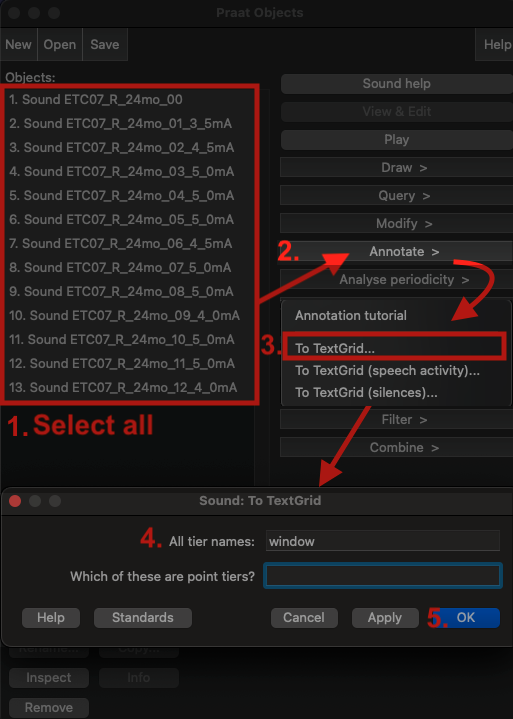
\includegraphics[width=3.64583in,height=\textheight]{img/praat-settings.png}
\caption{Screenshot of a step-by-step flowchart for how to create TextGrids for all audio files simultaneously.}
\end{figure}

\section{Creating TextGrids}\label{creating-textgrids}

Once the TextGrids are created, you will see a new file for each audio recording in the Praat Objects window. You want to select both the sound file and the TextGrid file for each recording. You can do this by holding down the \texttt{shift} key and clicking on the 2 files you want to select. Make sure that the sound file and the TextGrid file have the same name. A good way to check is to look at the configuration number in the file name. This will be a number between 00 and 15 and is located right after the timepoint (e.g., \texttt{12mo\_04}). If the sound file is \texttt{ETC07\_R\_12mo\_07\_5\_0mA}, the TextGrid file should be the same.

\begin{figure}
\centering
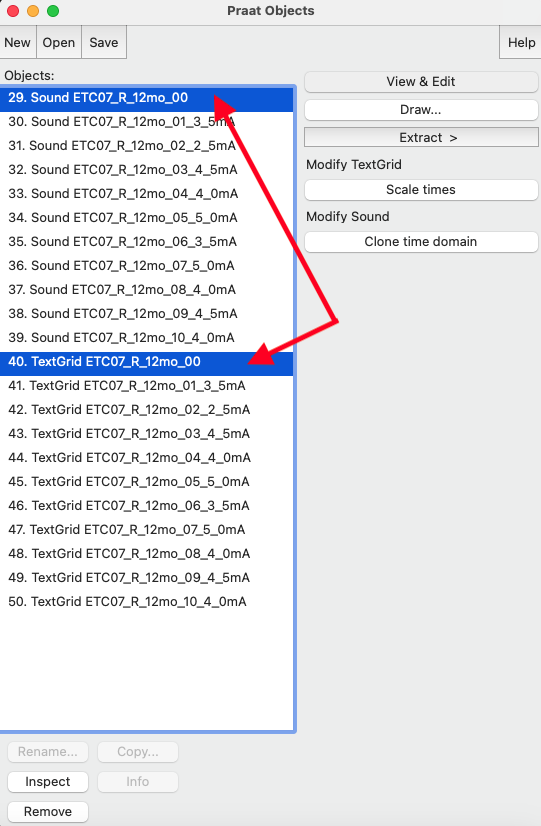
\includegraphics[width=3.64583in,height=\textheight]{img/praat-both-selected.png}
\caption{Screenshot of how to select both the sound file and the TextGrid file in Praat.}
\end{figure}

With both files selected, go to the right side and select View \& Edit. This will open a new window with the sound file and the TextGrid file.

\section{Viewing the files}\label{viewing-the-files}

The top two windows are audio file modules; the top window shows the waveform and the middle window shows the spectrogram. You will need to zoom in further to view the spectogram.

The TextGrid file is located in the bottom window. Off to the right you will see letters and symbols (not shown in screenshot). You can ignore these.

\begin{figure}
\centering
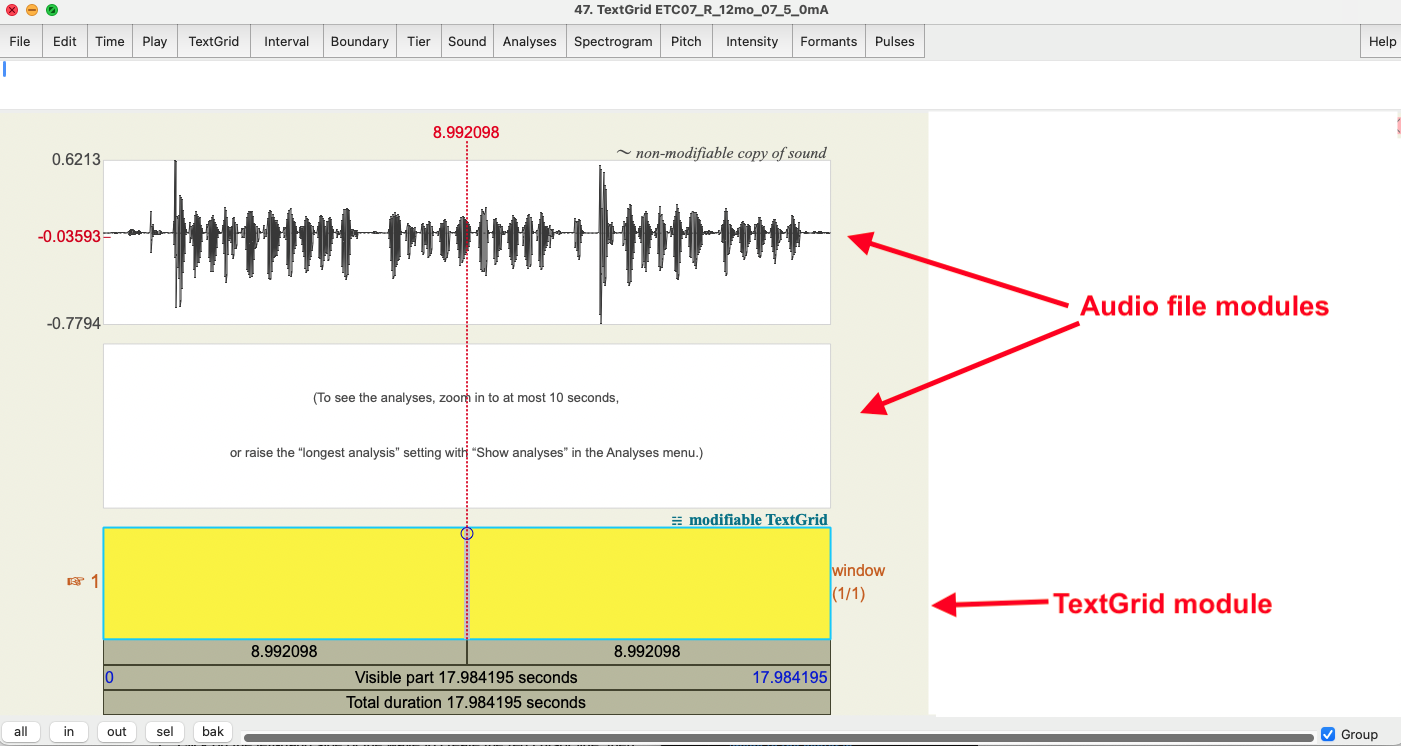
\includegraphics[width=5.20833in,height=\textheight]{img/praat-layout.png}
\caption{Screenshot of the Praat layout with the waveform, spectrogram, and TextGrid windows.}
\end{figure}

The waveform is helpful for seeing when the syllable begins and ends because it goes from a flat line to a wave and vice versa.

The spectrogram is helpful for fine tuning the beginning and end of the syllable. The tool shows the \href{http://www.phys.unsw.edu.au/jw/formant.html}{formants}, with the blue line indicating the base formant. Each formant corresponds to a resonance of the vocal tract (frequency at which the vocal folds are vibrating). The formants run horizontal, but when stacked, they look like dark black bands running vertically from the top to the bottom of the spectrogram window.

\begin{figure}
\centering
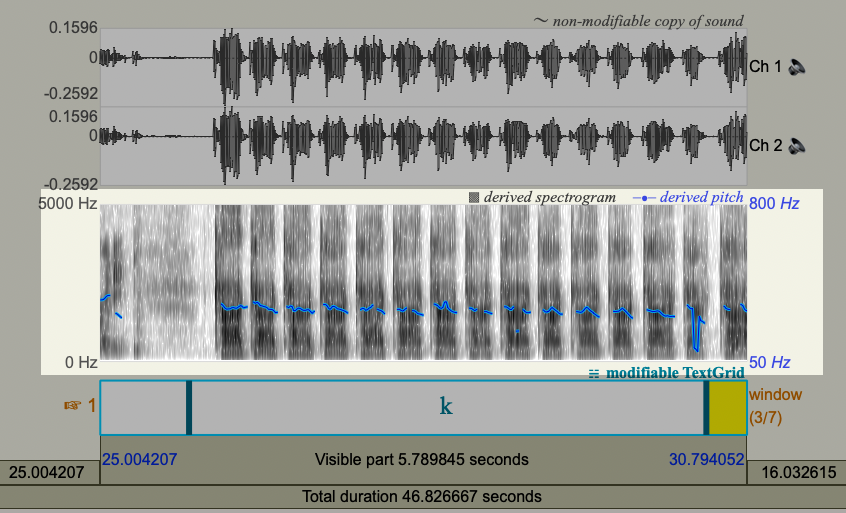
\includegraphics[width=5.20833in,height=\textheight]{img/praat-spectrogram.png}
\caption{Screenshot of the Praat spectrogram with the formants highlighted.}
\end{figure}

\section{Playing the audio file}\label{playing-the-audio-file}

Click on the left-hand side of the wave in the top window to move the red cursor line. Then click \texttt{tab}. This will play everything to the right of the cursor that is in the playable window.

To listen to a specific part of the audio file, click and drag the mouse over the waveform. Then click \texttt{tab} to play the selected portion.

There should be roughly 10 of each syllable, but listen to the recording to make sure you are analyzing the correct syllables.

\section{Defining the windows}\label{defining-the-windows}

Each TextGrid should be divided into 7 windows. The order of the windows is as follows:

\begin{enumerate}
\def\labelenumi{\arabic{enumi}.}
\item
  Cushion
\item
  Vowels (ka/)
\item
  Cushion
\item
  Vowels (ta/)
\item
  Cushion
\item
  Vowels (pa/)
\item
  Cushion
\end{enumerate}

The order could vary if the syllables are not recited in the order ka/ta/pa/. This will not affect the pipeline.

The three vowel windows should include all repetitions of each syllable. It is recommended to include a few milliseconds of silence before and after the syllable. This will help the pipeline identify the syllable.

The silence or background noise windows should cushion the vowel windows. There should be at least 4 of these windows.

Avoid overlapping windows. If you have overlapping windows, the pipeline will not work.

To define the windows, click on the waveform and drag the mouse to the right. This will define a window. If the window is too large or too small, click outside of the window and define a new area. To save the window, click \texttt{Interval} → \texttt{New\ interval\ on\ tier\ 1}.

\begin{figure}
\centering
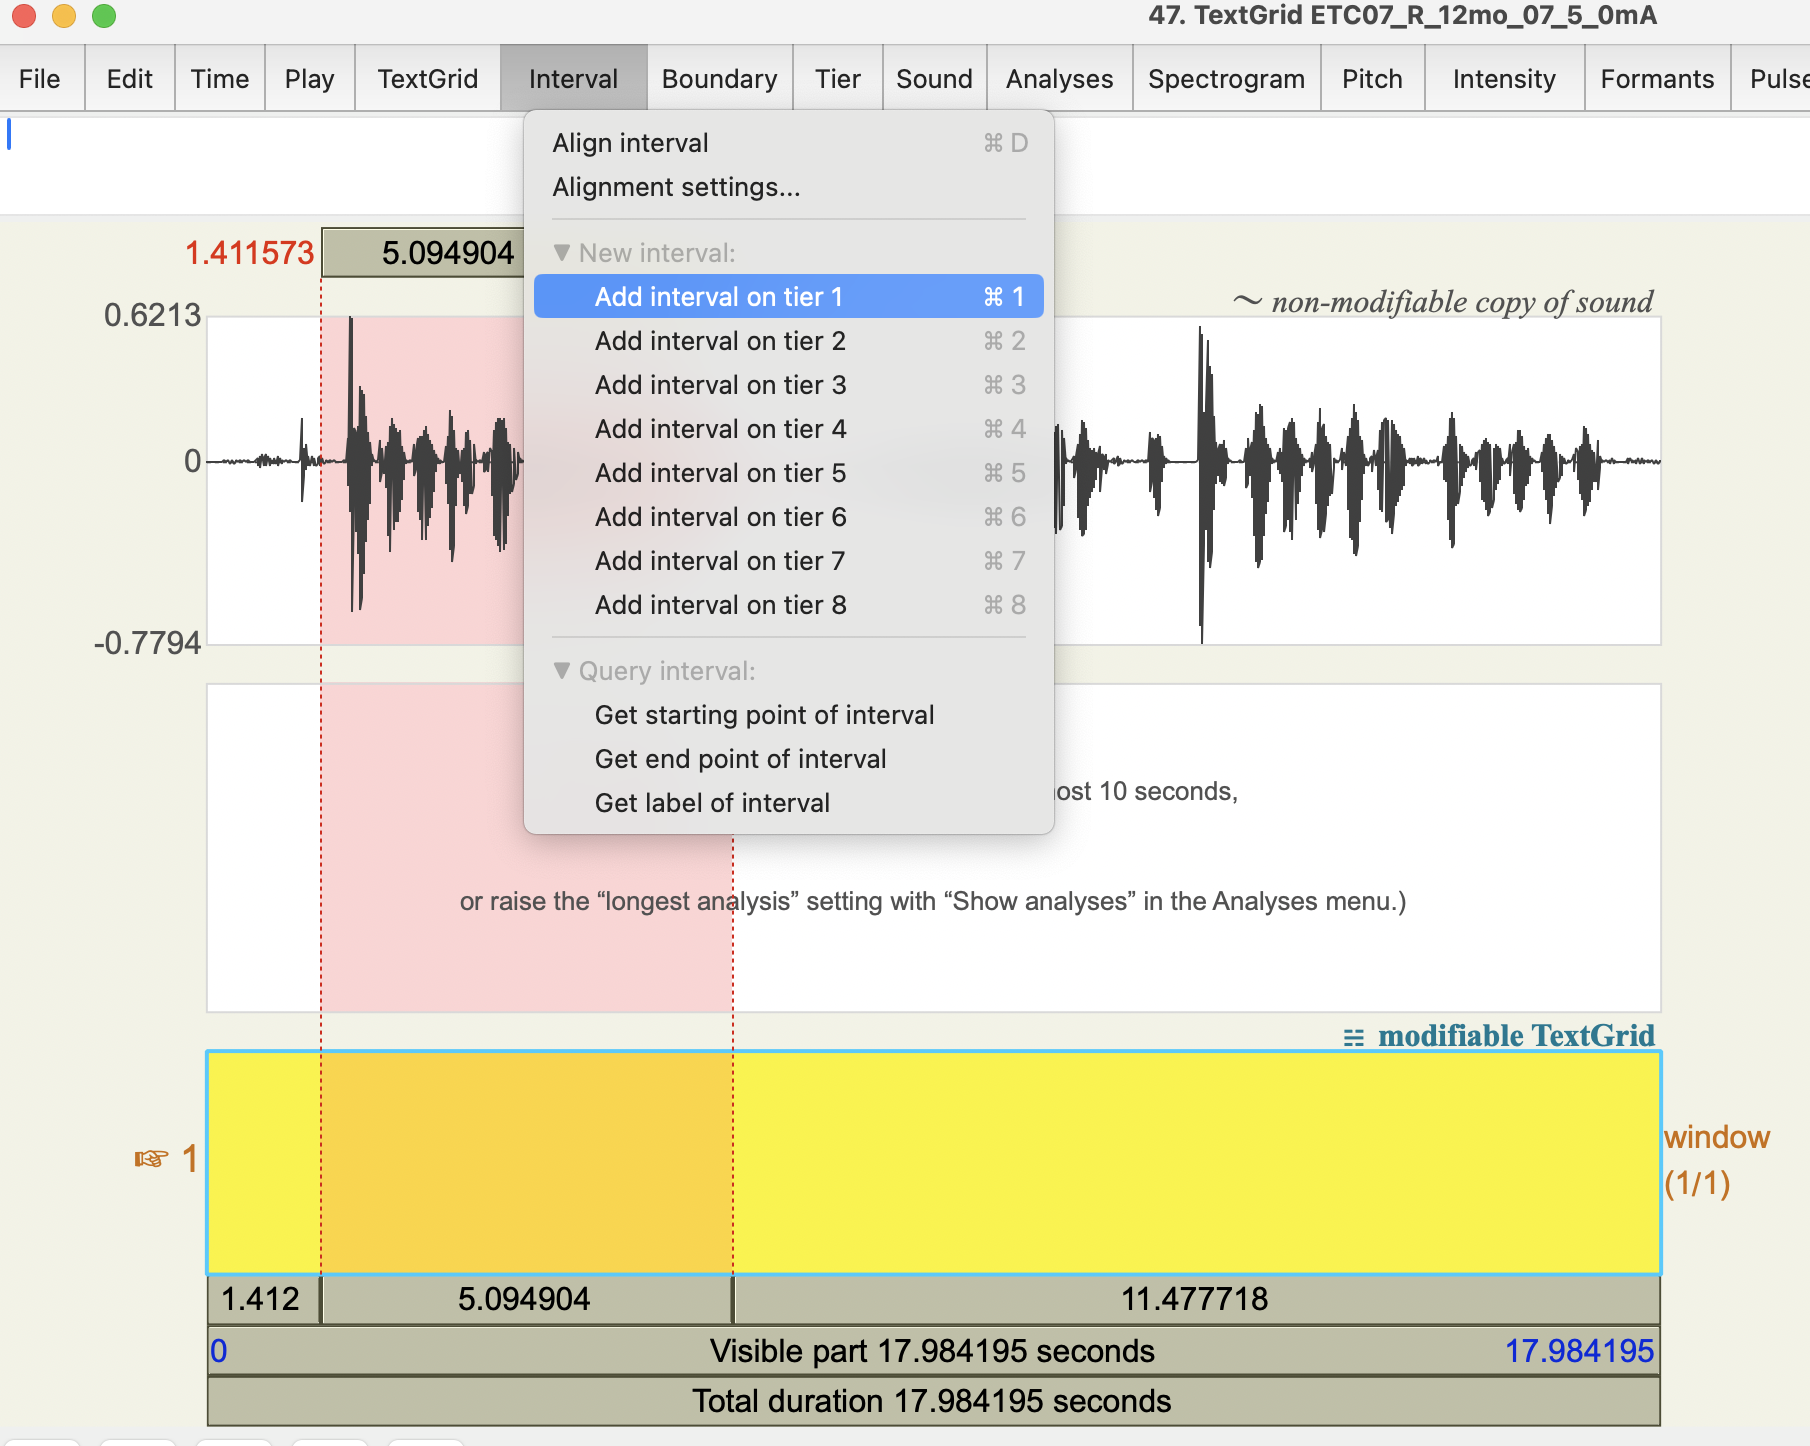
\includegraphics[width=5.20833in,height=\textheight]{img/praat-add-int.png}
\caption{\emph{Screenshot of how to add an interval in Praat.}}
\end{figure}

Once all the windows are defined, select each syllable interval and type either \texttt{k}, \texttt{t}, or \texttt{p}. This will label the interval with the corresponding syllable. Leave the cushion intervals blank.

Below is a screenshot of what the TextGrid should look like when it is complete. Check that in the bottom left you see \texttt{window\ (\#/7)}.

\begin{figure}
\centering
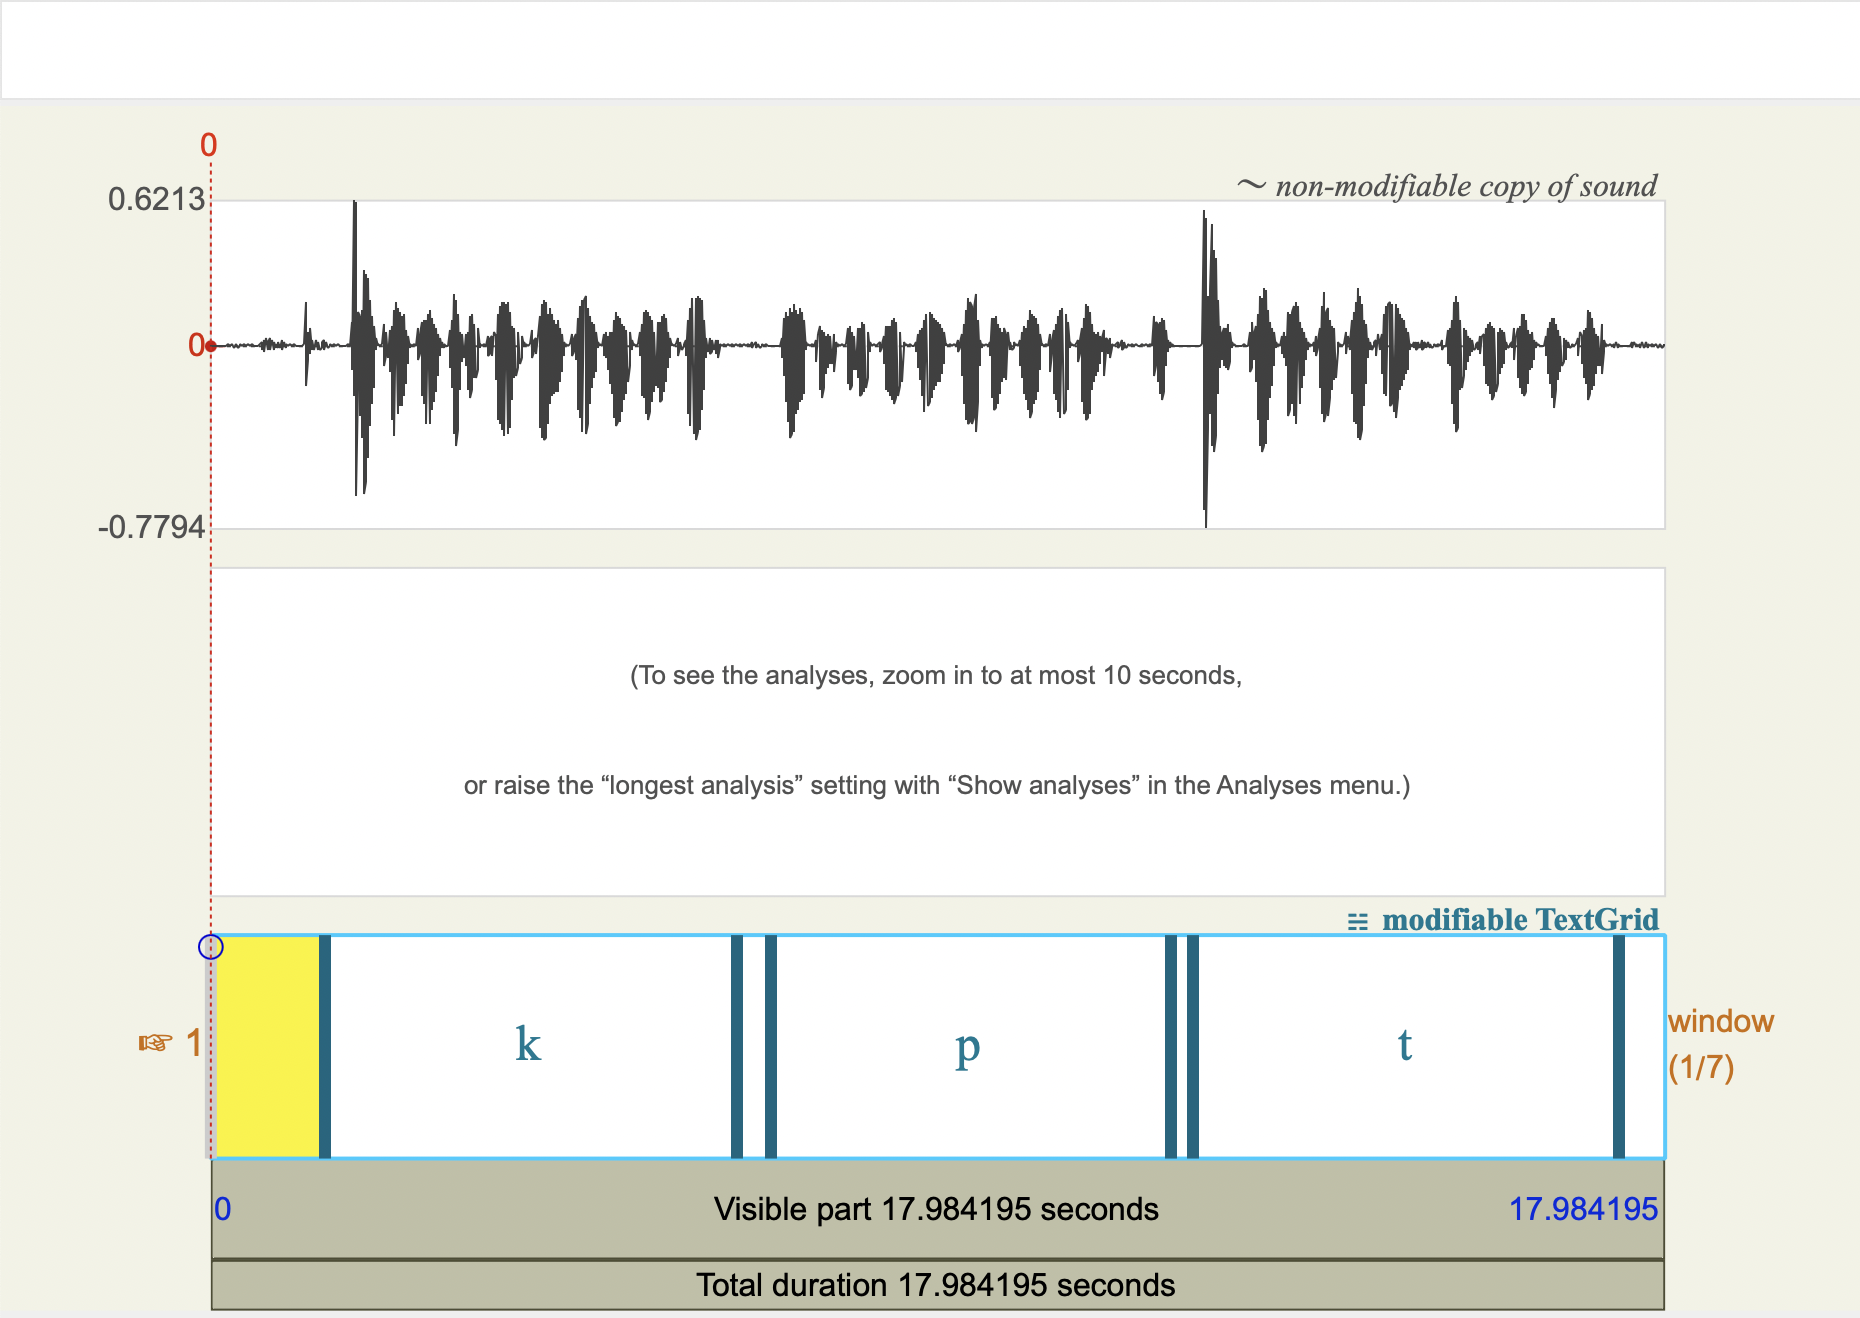
\includegraphics[width=5.20833in,height=\textheight]{img/praat-final.png}
\caption{Screenshot of a completed TextGrid with 7 windows.}
\end{figure}

\section{Saving the TextGrid}\label{saving-the-textgrid}

Before you close the window, save the TextGrid by going to \texttt{File} → \texttt{Save\ as\ text\ file}. \textbf{Save the file in the same folder as the audio file.} The file should have the same name as the audio file with the extension \texttt{.TextGrid}. In order for the pipeline to work, the TextGrid file must be saved in the same folder as the audio file AND have the exact same name as the audio file.

Now, repeat this process for all of the audio files in the folder that you want to analyze.

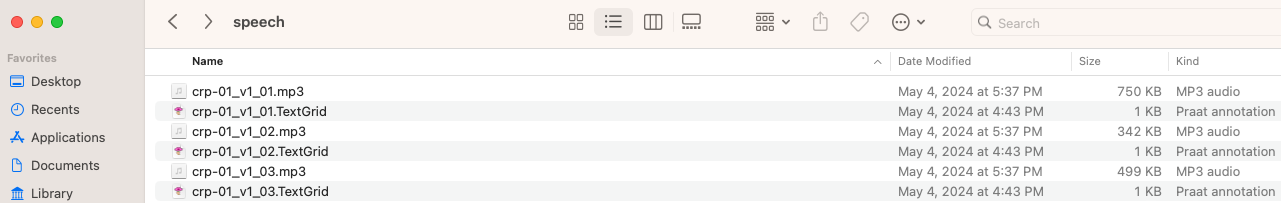
\includegraphics[width=8.33333in,height=\textheight]{img/praat-filenames.png}
\hyperref[working-with-praat]{To top of page ↑}

\chapter{Preprocessing data}\label{preprocessing-data}

\section{\texorpdfstring{Clear out the \texttt{ddktor-dbs/data/raw} folder using \texttt{clear\_raw.py}}{Clear out the ddktor-dbs/data/raw folder using clear\_raw.py}}\label{clear-out-the-ddktor-dbsdataraw-folder-using-clear_raw.py}

Before running the preprocessing scripts, ensure that the \texttt{ddktor-dbs/data/raw} folder is empty. This folder is where the audio files and corresponding TextGrid files will be transferred to after running the \texttt{mp3\_to\_wav.py} script.

You can easily clear out the \texttt{ddktor-dbs/data/raw} folder by running the following command from the \texttt{ddktor-dbs} directory: \texttt{python3\ clear\_raw.py} This script will delete all files in the \texttt{ddktor-dbs/data/raw} folder.

\section{\texorpdfstring{Run \texttt{m4a\_to\_mp3} (if needed)}{Run m4a\_to\_mp3 (if needed)}}\label{run-m4a_to_mp3-if-needed}

Before running the \texttt{mp3\_to\_wav.py} script, you may need to convert your audio files from m4a to mp3 format. If your audio files are in m4a format, you can convert them to mp3 format before running the \texttt{mp3\_to\_wav.py} script.

It will ask you for the root directory containing the m4a files to convert. Press Enter to use the default directory. It will then ask you for a subdirectory or multiple subdirectories (separated by commas) of \texttt{data/raw/} containing m4a files to convert. Enter them as a comma-separated list. An example is provided in the prompt.

An example input is provided below:

\texttt{crp-01/visit2/speech}

\section{\texorpdfstring{Run \texttt{mp3\_to\_wav.py}}{Run mp3\_to\_wav.py}}\label{run-mp3_to_wav.py}

DDKtor requires all audio files to be in wav format. If your audio files are in mp3 format, you can convert them to wav format.

A script titled \texttt{mp3\_to\_wav.py} is provided in the \texttt{pipeline} folder. This script will convert all mp3 files in the \texttt{data} folder to wav files. Additionally, it will transfer these wav files to the \texttt{ddktor-dbs/data/raw} folder along with the corresponding TextGrid files. In order for this script to run, ALL files must be organized in the following manner:

\begin{itemize}
\tightlist
\item
  All files must be located in the \texttt{data/raw/} folder.\\
\item
  All files must be in the format \texttt{subjectID\_visitID\_instanceID.mp3} (e.g., \texttt{crp-01\_v1\_01.mp3})

  \begin{itemize}
  \tightlist
  \item
    Don't forget the leading zero for single-digit instance subject and instance IDs.
  \end{itemize}
\item
  All files must have a corresponding TextGrid file in the format \texttt{subjectID\_visitID\_instanceID.TextGrid} that is \textbf{exactly the same} as the audio file. (e.g., \texttt{crp-01\_v1\_01.TextGrid})
\end{itemize}

Ensure your data is organized in a similar manner to the following:

\begin{verbatim}
data
├── raw
│   ├── crp-01
│   │   ├── visit1
│   │   │   ├── speech
│   │   │   │   ├── crp-01_v1_01.mp3
│   │   │   │   ├── crp-01_v1_01.TextGrid
│   │   │   │   ├── (...)
│   │   ├── visit2
│   │   │   ├── speech
│   │   │   │   ├── crp-01_v2_01.mp3
│   │   │   │   ├── crp-01_v2_01.TextGrid
│   │   │   │   ├── (...)
│   ├── crp-xx
│   │   ├── visitx
│   │   │   ├── speech
│   │   │   │   ├── crp-xx_vx_0x.mp3
│   │   │   │   ├── crp-xx_vx_0x.TextGrid
│   │   │   │   ├── (...)
(...)
\end{verbatim}

To run the script, navigate to the \texttt{pipeline} folder and run the following command: \texttt{python3\ mp3\_to\_wav.py}. The script will prompt you for several inputs:

\begin{enumerate}
\def\labelenumi{\arabic{enumi}.}
\tightlist
\item
  \texttt{Please\ enter\ the\ root\ directory\ containing\ mp3\ files\ to\ convert.\ Press\ Enter\ to\ use\ the\ default\ directory.}: Press Enter to use the default directory.
\item
  \texttt{Please\ enter\ a\ subdirectory\ or\ multiple\ subdirectories\ (separated\ by\ commas)\ of\ ../../data/raw/\ containing\ mp3\ files\ to\ convert.\ Example:\ crp-01/visit2/speech,crp-03/visit5/speech}: Enter one or more subdirectories containing the mp3 files you would like to convert. Enter them as a comma-separated list. An example is provided in the prompt.
\item
  You should see a message indicating that the script is converting the mp3 files to wav files. Each file will either be successfully converted or an error message will be displayed.
\item
  Once the script has finished running, you should see a green message indicating \texttt{All\ conversions\ are\ complete\ and\ have\ been\ saved\ to\ DDKtor.}
\item
  Importantly, it should also display a message indicating \texttt{TextGrid\ files\ have\ also\ been\ transferred\ to\ DDKtor.} Make sure that the number of TextGrid files transferred matches the number of wav files transferred.
\end{enumerate}

\begin{figure}
\centering
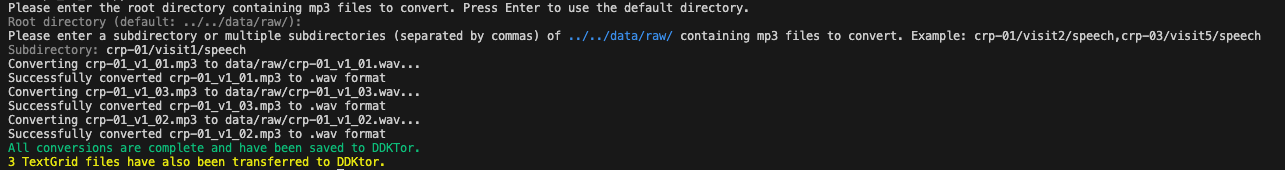
\includegraphics[width=5.20833in,height=\textheight]{img/preprocess-transfer.png}
\caption{Screenshot of a successful pre-processing script run.}
\end{figure}

Now, navigate to the \texttt{ddktor-dbs/data/raw} folder and ensure that all of the wav files and corresponding TextGrid files have been transferred successfully.

\section{\texorpdfstring{Run \texttt{match.py} (optional)}{Run match.py (optional)}}\label{run-match.py-optional}

If you have a large number of files and would like to ensure that all audio files have corresponding TextGrid files, you can run the \texttt{match.py} script. This script will check for any audio files that do not have corresponding TextGrid, or vice versa. If any files are missing, the script will display a message indicating which files are missing. It also returns the number of matches.

This step is not required, but it can be helpful to ensure that all files have been transferred successfully.

\chapter{DDKtor}\label{ddktor}

Once you have all raw data in \texttt{ddktor-dbs/data/raw}, you are ready to run the DDKtor pipeline.

\begin{enumerate}
\def\labelenumi{\arabic{enumi}.}
\tightlist
\item
  Make sure your working directory is \texttt{ddktor-dbs}.
\item
  Run the following commands to check installation and run the pipeline:

  \begin{itemize}
  \tightlist
  \item
    \texttt{chmod\ +x\ check\_installations.sh}
  \item
    \texttt{./check\_installations.sh}
  \end{itemize}
\item
  If everything is correctly installed, the terminal will print \texttt{All\ good\ :)}
\item
  Run the main shell script:

  \begin{itemize}
  \tightlist
  \item
    \texttt{\$\ chmod\ +x\ ./run\_script.sh}
  \item
    \texttt{./run\_script.sh}

    \begin{itemize}
    \tightlist
    \item
      To process with noise reduction, run \texttt{./run\_script.sh\ -n}
    \end{itemize}
  \end{itemize}
\end{enumerate}

A successful run should look like the following:
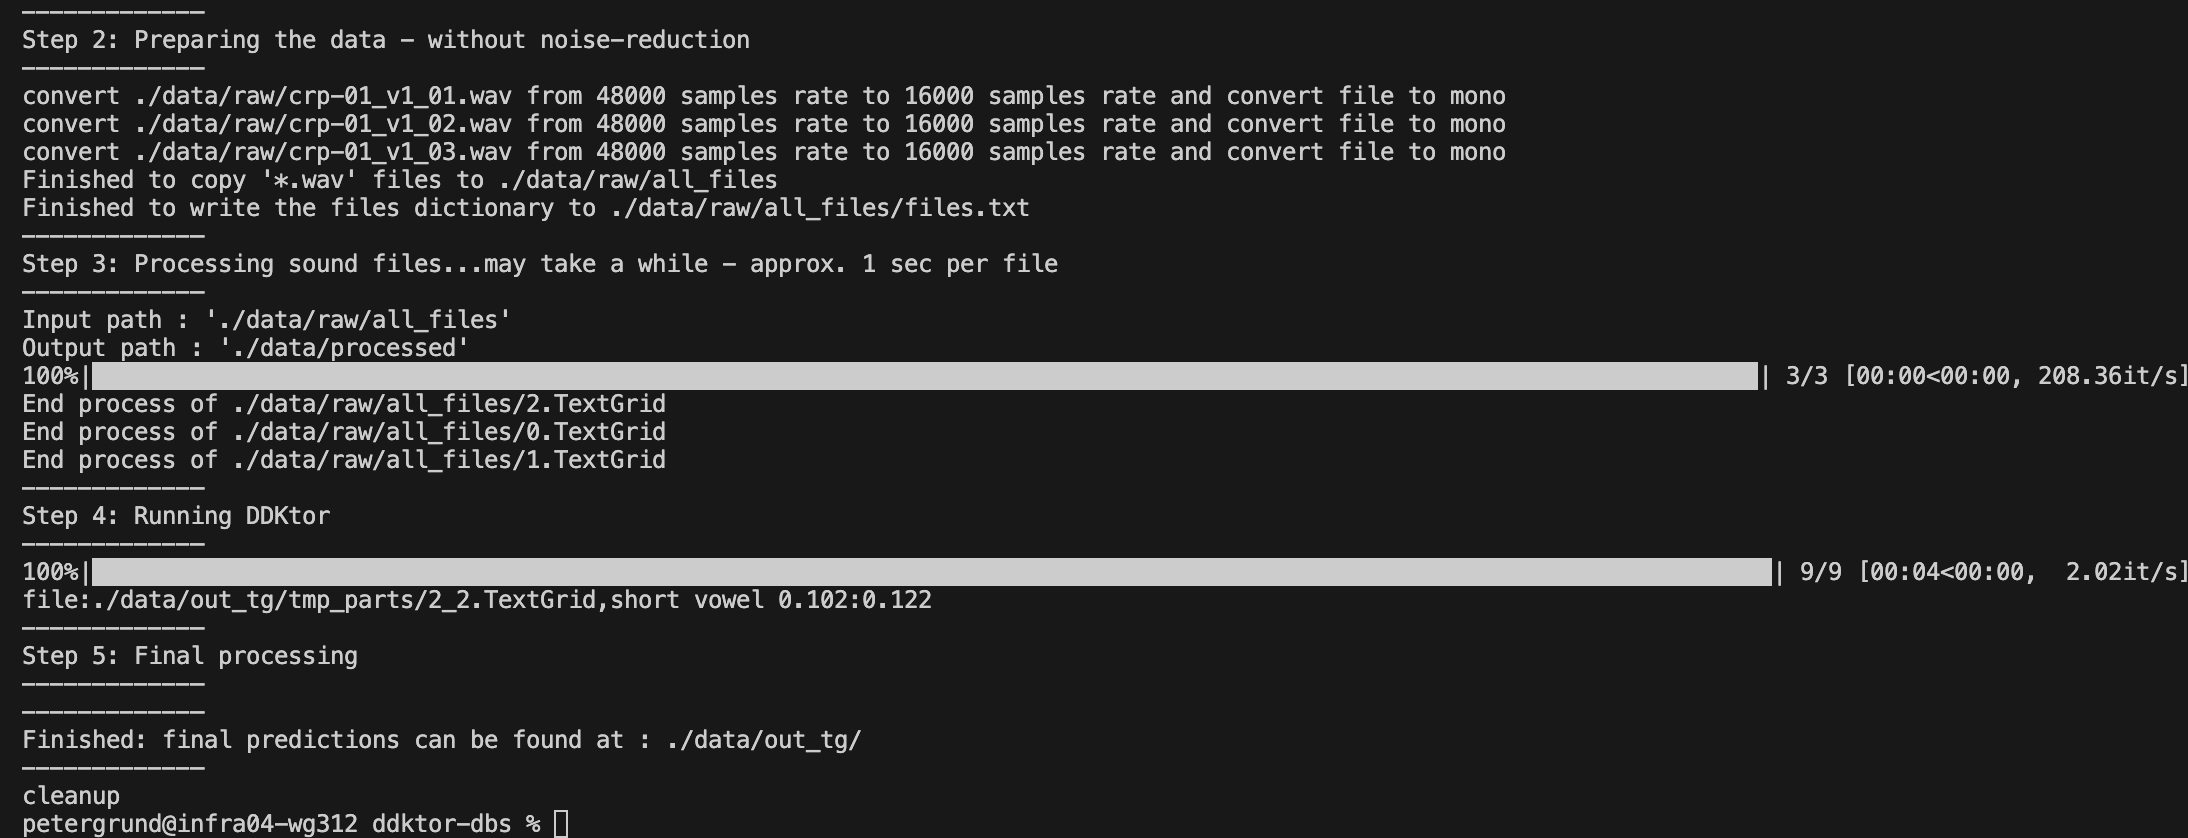
\includegraphics[width=5.20833in,height=\textheight]{img/ddktor-success.png}

If you encounter errors saying that certain packages are missing, install them by typing into the terminal \texttt{pip\ install\ {[}package{]}} without the brackets.

\chapter{Post-processing}\label{post-processing}

Once DDKtor has finished running, check to see if new \texttt{.textgrid} files have been saved in \texttt{data/out\_tg}. Make sure there are as many output files as you're expecting.

Next, the \texttt{.textgrid} files need to be converted to \texttt{.csv} for analysis.

To do this, run \texttt{textgrid\_to\_csv.py}. The script will do the following:
* It starts by setting up a temporary folder (mid/) to hold intermediate files during processing.
* The reads .TextGrid files from the output directory, extracts key speech intervals (letters and timing details), and saves them as .csv files.
* It standardizes the data by renaming columns for clarity, adding metadata (like study ID or visit number) from filenames, and cleaning up text entries (e.g., fixing letter formats).
* Next, it pairs specific intervals (e.g., VOT and vowel segments), calculates their durations, and organizes them into a single dataset with additional details like sequence order.
* Finally, it combines all the processed data into one CSV file, names it based on the study ID (e.g., STUDY\_ID\_merged\_\#.csv), and removes the temporary folder.

You can find the finished \texttt{.csv} file in \texttt{CR-DBS\_for\_ET\_UH3/data/processed/speech/csv\_files}.

  \bibliography{book.bib,packages.bib}

\end{document}
